%%% -*-LaTeX-*-

\chapter{Introduction}
\label{ch:introduction}
From the cosmic scale of astronomy to the atomic scale of chemistry, and from speculative economics to precision engineering, experts in a variety of fields are interested in gathering data in order to better understand the functional relationships between target quantities of interest and their presumed driving forces.
%
For instance, what chemical or structural characteristics of a nuclear fuel optimize its safety and efficiency and to what degree and under what conditions?
%
Or to take an example from a different field, what socioeconomic factors play the largest role in determining quality of life?
%
For abstract notions such as ``safety'' and ``quality of life'' that can be encoded numerically and measured or simulated, the scientific community has been designing analysis tasks capable of answering these types of questions.
%
Such tasks include identifying parameters of interest from a field of candidates, efficient collection of data relating the candidate parameters to the outputs, identifying and summarizing trends in the functional relationship of the input space and output space, and building efficient and reliable predictive models.

However, many new and yet unexplored ideas lie at the intersection of fields of study such as statistics, geometry, and visualization.
%
Therefore, it is important to apply validated ideas from these disparate fields in order to augment and enhance solutions to problems occurring in other areas.
%
By combining complementary techniques, we can gain a new understanding about our observed data and even inform the data gathering process.
%
One such field of recent interest is topological data analysis (TDA).
%
TDA is a growing field arising from the combination of computational geometry, topology, set theory, and visualization.

In this work, I investigate the efficacy of TDA techniques to problems arising in the realm of uncertainty quantification and risk monitoring.
%
In particular, I place a special emphasis on applications relevant to nuclear safety, such as adaptive sampling, sensitivity analysis, regression, limit surface extraction, and visualization of risk-informed datasets.
%
\textit{By approximating topological constructs from potentially sparsely sampled data, we are able to extract and analyze the structure of scientific simulation data stemming from low (one to three) to moderate (on the order of tens) dimensional input spaces to provide actionable insight for domain scientists.}

This introductory chapter will qualify what kind of data this work applies to and will introduce the specific problem domain areas.
%
Chapter~\ref{ch:definitions} will normalize our language by synthesizing the relevant information from several fields, including data analysis, set theory, algebra, topology, and graph theory.
%
Chapter~\ref{ch:related} frames the contributions of this work in the context of related research and the current state of the art.
%
Chapter~\ref{ch:theory} addresses the theoretical aspects of the work involved by giving a thorough background on the topological constructs used throughout this body of research.
%
Chapters~\ref{ch:adaptiveSampling} and~\ref{ch:visualization} elaborate on novel solutions to problems in adaptive sampling and analysis of generated data.
%
Lastly, Chapter~\ref{ch:graphs} presents an in-depth study of the approximation quality of constructs presented in earlier chapters by enhancing and evaluating the underlying graph structures used for performing various analyses.

\section{Scientific Discovery Through Exploratory\\Data Analysis}

We, as scientists, advance the state of the art by application of the scientific method, which typically begins with an observation that leads to a hypothesis.
%
A reproducible experiment is designed to test the hypothesis in a controlled environment.
%
Data from the experimental phase is then analyzed in order to reject, amend, or accept the tested hypothesis whereupon follow-up experiments can be done to further validate or strengthen a proposed hypothesis.
%
It may seem trivial to mention such a basic tenant of the scientific discovery process, but it will serve as a basis for the problems being addressed in this dissertation that aims at alleviating issues occurring in this process in a generically applicable fashion.
%
Thus, the components of this body of research have a wide range of applicability to disparate fields of science, all applying this methodology.

\begin{figure}[t]
  \centering
  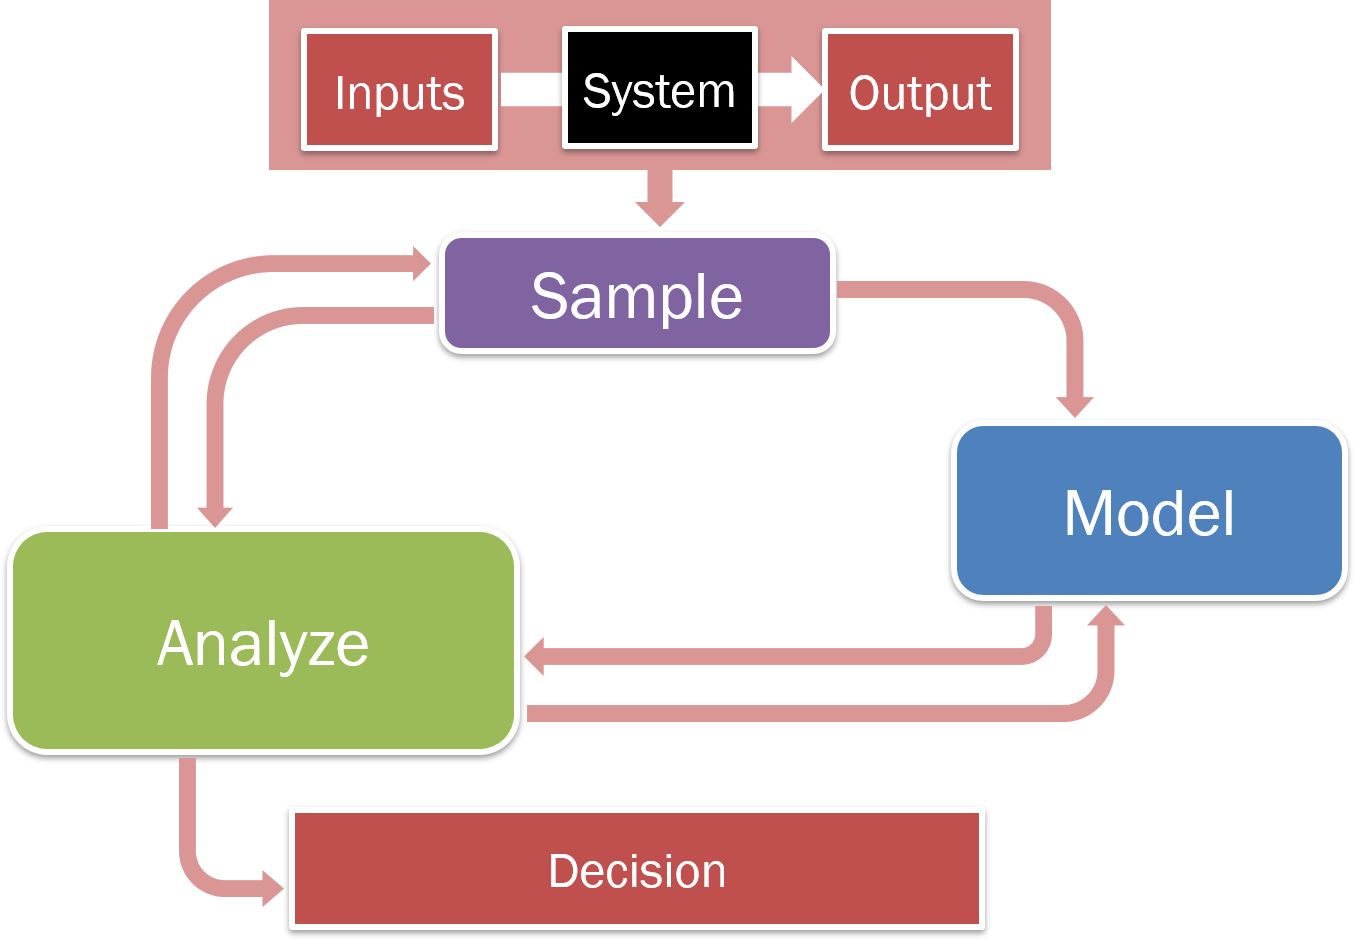
\includegraphics[width=.65\textwidth]{figs/chap1/pipeline}
  \caption[Data collection cycle for scientific discovery]{A broad view of the exploratory data analysis pipeline under study.}
  \label{fig:dataCycle}
\end{figure}

Figure~\ref{fig:dataCycle} shows a summary of the exploratory data pipeline that we are considering.
%
The pipeline begins with the top box where we must first identify what quantities of interest we are going to observe.
%
Note that the inputs and outputs may not be clearly defined at this point, but the important aspect is that we are identifying a superset of the relevant quantities to be measured in our experimentation phase.
%
Often during initial analysis, we may cast a wider net than needed, and so in later phases we may refine or reduce the set of inputs and targets.
%
In this body of work, we will be looking at experimental numeric data collected from various domains.
%
An experiment in our context is a procedure used to validate or invalidate some hypothesis set forth by the domain scientist.
%
The hypothesis usually seeks to define a relationship among different variable factors in a system under study.
%
A simulation is simply a computer experiment, i.e., a repeatable procedure with one or more variable input factors executed in a computational environment that produces one or more output factors to be analyzed.
%
Most of the applications in this work will be on simulations and not physical experiments, although from our standpoint, the difference is negligible because the methods described herein apply equally to both.
%
Therefore, we will use the term \textit{experiment} in order to be as general as possible.
%
In order to perform an experiment, we typically perform the procedure under different settings for a set of factors we believe to be significant.
%
Let us illustrate with an example.

In the scenario introduced above regarding nuclear fuel design, the first task for the scientist is to quantify what denotes a ``safe'' fuel.
%
Next, the scientist will design one or more canonical scenarios by which to evaluate the safety of the fuel.
%
In designing these scenarios, the scientist is building a hypothesis about the factors that will affect the fuel's safety.
%
In the case where the factors can be quantified, the scientist will likely utilize some variation of the loop from Figure~\ref{fig:dataCycle}.
%
The scientist will thus generate and analyze data with the end goal of making a decision.
%
In this case, the decision may be to pursue a particular type of fuel for use in production or to use an approximation for more extensive testing at a reduced cost.

We specifically target multidimensional, numeric data that can be modeled as a scalar function.
%
A scalar function simply means that for a set of input parameters, we associate a single target output value.
%
Multidimensional, in this setting, is taken to mean that the collection of inputs associated to the target value consists of two or more numeric values.
%
With this defined context, we proceed to the sampling phase of the process.

\subsection{Data Sampling}

The collection of quantities being measured define a multidimensional space, and in order to perform any analysis, we must first collect some amount of data in this space.
%
Sampling, or data collection, ranges anywhere from a dense sampling of the entire space of interest down to collecting only a handful of sparsely available observations or anything in between.
%
For instance, in many low dimensional (read two or three) simulation examples, we may rely on a very fine or possibly adaptively refined grid of data to observe the specific characteristics of a phenomenon or utilize experimental designs for response surface methodology which can be used to interpolate between grid cells.
%
In higher dimensional cases, it can often be infeasible to perform such a dense sampling due to the immensity of the space being considered, and so we rely on space-filling designs or adaptive sampling strategies to place samples in the most perceived important areas.
%
Space-filling methods attempt to balance randomness with sampling density.
%
We review such space-filling techniques in Section~\ref{sec:forwardSampling}.
%
On the other hand, acknowledging that only a potentially small subspace of the input domain is interesting has led to the development of several adaptive algorithms that iteratively refine our understanding of the input space through careful selection of input samples.
%
The selection process is usually driven by an underlying model of the data that may favor areas of high uncertainty, steep gradient, low density, or optimized values.
%
We review adaptive sampling techniques in Section~\ref{sec:adaptiveSampling}.
%
I present novel methods for injecting topology into the scoring and selection of candidates in the adaptive sampling process in Chapter~\ref{ch:adaptiveSampling}.
%
In other cases, our hands may be tied to use whatever data is available.
%
This latter case is more common in physical observation tasks where, for example, instrumentation may be limited to specific geospatial locations.
%
Once data has been collected we may either elect to directly analyze the data or build a model of the data which allows us to characterize unobserved areas of the domain.

\subsection{Data Modeling}

The modeling phase includes things like classifiers, regressors, structural models, statistical models, and reduced order models.
%
Classifiers and regressors, or more generically, predictors connect the input space to one or more target outputs by generating labels or real values, respectively.
%
The latter three types of models can be special cases of predictors, but may also provide additional information.
%
For instance, a structural model could be a graph that connects the underlying samples thus imposing a specific manifold geometry that is different than the embedding space in which the data resides.
%
Statistical and ensemble models can be used to add more contextual information such as incorporating uncertainty into a model's prediction.
%
Lastly, reduced order modeling can be a simpler mathematical model that can be used as a significantly more efficient proxy for generating more data or can more succinctly summarize the global behavior of a system.

I summarize several common classes of data modeling in Section~\ref{sec:regression}.
%
These data modeling methods are used heavily in the novel works of Chapters~\ref{ch:adaptiveSampling} and~\ref{ch:visualization}.
%
In Chapter~\ref{ch:graphs}, I specifically look at different structural models and their suitability for multidimensional data analysis.
%
In this chapter, I generalize existing graph models and provide a unified framework for efficiently approximating various graph types by exploiting graphical processing unit (GPU) parallelism.
%
Once we have constructed a model from the existing data, we move to the analysis phase.

\subsection{Data Analysis}

As noted in Figure~\ref{fig:dataCycle}, we can arrive at or can move from the analysis phase from any other phase in the data lifecycle making it one of the most crucial aspects of data exploration.
%
For example, we may directly evaluate the suitability of a given sample set of data and decide that more data is needed before any decision can be made.
%
Alternatively, given a particular model and data fit to it, we may evaluate its efficacy for a given problem and determine that it does not capture the behavior we expect and iterate between the modeling and analysis phases until we arrive at a suitable model.
%
The ultimate goal however is to synthesize the data collected and potentially a suitable model into a decision through analysis.
%
Examples of analysis include studying statistics of the gathered data possibly broken into meaningful partitions or clusters, computing correlations among inputs and between inputs and outputs, understanding sensitivity information regarding different experiment parameters, and generating visualizations to augment the study of all of the above.
%
These techniques are reviewed in Chapter~\ref{ch:related}.
%
In Chapter~\ref{ch:visualization}, I highlight novel, published work that explores the use of topological techniques for performing structured sensitivity analysis within a visualization system designed specifically for nuclear engineers.
%
This work is incorporated into the RAVEN software~\cite{RabitiAlfonsiCogliati2015}, developed at Idaho National Laboratory and is currently used by nuclear engineers for analyzing experimental results ranging from nuclear fuel design to multiplant coordination.

% \bibliography{\jobname}